\chapter{Introduction}
\label{chap:Introduction}

In the introduction section, you should discuss the topic you plan to research in your seminar. Pay attention to the following points:
\begin{dinglist}{52}
\item Be sure to clearly explain the area of work and the problem you intend to address,
\item Describe the existing challenges in the field you are focusing on in detail,
\item Ensure to reference credible articles and sources,
\item Use high-quality images where appropriate. If you use an image from another source, make sure to properly reference it. For example please see \autoref{fig:RBConcept}.
\item Please define your abbrevation in './ETC/abbr'  file, and use it in your report by using  'gls' command such as \gls{GIS}.
\end{dinglist}
\begin{figure}
\centering
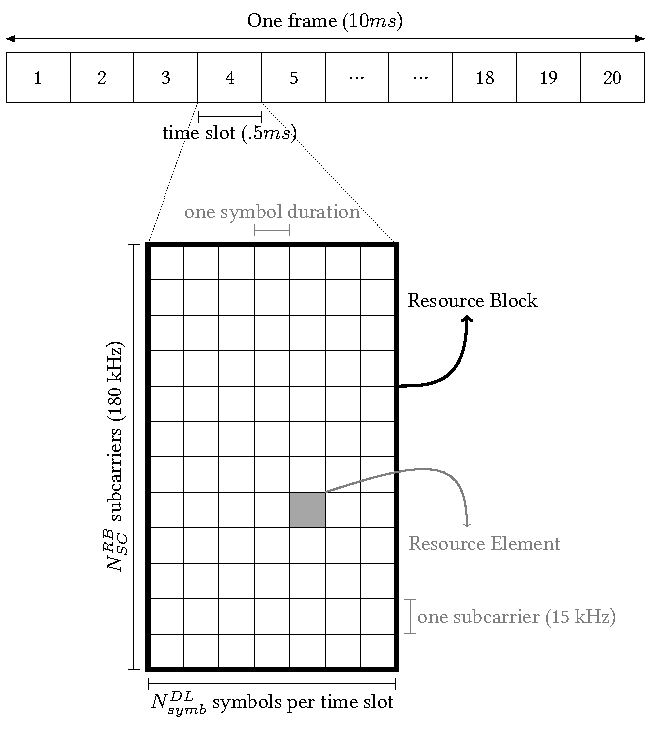
\includegraphics[width=0.6\linewidth]{./Pic/RBConcept/mainFig}
\caption{\lofimage{./Pic/RBConcept/mainFig}%
Resource block and resource element concept in LTE \cite[Fig. 3.2.3]{Rumney2013LTE}.}
\label{fig:RBConcept}
\end{figure}

\section{Problem Statement}
The problem statement outlines the specific issue or challenge that your research aims to address. It provides a clear and concise description of the gap or deficiency in the current knowledge or practice that your study seeks to fill. This section highlights the significance of the problem and sets the foundation for why your research is necessary. Key points for writing a problem statement:
\begin{enumerate}
\item Clearly define the issue or challenge.
\item Explain the impact or consequences of the problem if left unresolved.
\item Discuss any existing solutions or approaches and why they are insufficient.
\item Provide context by referencing relevant literature or real-world examples.
\end{enumerate}
Example: ``In recent years, there has been an increasing focus on improving energy efficiency in smart homes. However, current systems lack advanced automation capabilities for optimizing energy consumption based on real-time data. This research aims to address this gap by developing a smart energy management system that integrates machine learning for dynamic energy optimization."

\section{Research Objectives}
The research objective outlines the specific goals that the study intends to achieve. These objectives provide a roadmap for your investigation and guide the direction of your research. They should be clearly stated and measurable, allowing for an evaluation of the study's success.

Key points for writing research objectives:
\begin{enumerate}
\item Define clear and achievable goals.
\item Align objectives with the problem statement.
\item Specify whether the objectives are exploratory, descriptive, or explanatory.
\item Break down the main objective into smaller, specific objectives if needed.
\end{enumerate}
Example: ``The primary objective of this research is to develop a smart energy management system for homes that optimizes energy consumption using machine learning. The specific objectives include:
\begin{dinglist}{43}
\item Analyzing current energy management systems in the market.
\item Designing a machine learning algorithm for real-time energy optimization.
\item Testing and evaluating the performance of the developed system in a simulated environment."
\end{dinglist}


\section{Scope and Limitations}
The scope defines the boundaries of your research, outlining what will and will not be covered in the study. This helps set expectations for the reader. The limitation section, on the other hand, addresses any constraints or restrictions that may affect the study’s results or generalizability.

Key points for writing \textit{scope}:
\begin{enumerate}
\item Specify the aspects of the topic you will focus on.
\item Define the time frame, location, and sample size (if applicable).
\item Mention any specific variables or factors you will investigate.
\end{enumerate}

Key points for writing \textit{limitations}:
\begin{enumerate}
\item Identify any constraints like limited data, time, or resources.
\item Explain how these limitations might affect your results.
\item Be transparent about what the research cannot address or solve.
\end{enumerate}
Example for \textit{Scope}: ``This study focuses on developing a smart energy management system specifically for residential homes. It will use machine learning algorithms to optimize electricity usage based on data from energy consumption sensors. The system will be tested in a simulated environment rather than in real homes."

Example for \textit{Limitations}: ``This research is limited by the use of simulation for testing, which may not fully reflect real-world conditions. Additionally, the system will only address electricity usage and will not optimize other forms of energy consumption, such as heating or water usage."



\section{Structure of the Report}
The remaining sections of this document are structured as follows.  At the first step, in  \autoref{chap:Concepts}, we will explain the definitions and concepts related to our topics. Then, in \autoref{chap:RelatedWork}, we will review the previous works done in this field. Finally, in \autoref{chap:Conclusion}, we will summarize and conclude.







